% Modelo de Trabalho Acadêmico do curso de Engenharia da Computação em conformidade com
% ABNT NBR 14724:2011: Informação e documentação - Trabalhos acadêmicos 
% Autor Tiago Alves de Oliveira
% ------------------------------------------------------------------------
% ------------------------------------------------------------------------

\documentclass[
	12pt,				% tamanho da fonte
	openright,			% capítulos começam em página ímpar (insere página vazia caso preciso)
	oneside,			% para impressão em verso e anverso. Oposto a oneside
	a4paper,			% tamanho do papel. 
	brazil				% o último idioma é o principal do documento
	]{abntex2}

% ---
% Pacotes básicos 
% ---
\usepackage{lmodern}			% Usa a fonte Latin Modern			
\usepackage[T1]{fontenc}		% Selecao de codigos de fonte.
\usepackage[utf8]{inputenc}		% Codificacao do documento (conversão automática dos acentos)
\usepackage{lastpage}			% Usado pela Ficha catalográfica
\usepackage{indentfirst}		% Indenta o primeiro parágrafo de cada seção.
\usepackage{color}				% Controle das cores
\usepackage{graphicx}			% Inclusão de gráficos
\usepackage{microtype} 			% para melhorias de justificação
% ---
		
% ---
% Pacotes adicionais, usados apenas no âmbito do Modelo Canônico do abnteX2
% ---
\usepackage{lipsum}				% para geração de dummy text
% ---

% ---
% Pacotes de citações
% ---
\usepackage[brazilian,hyperpageref]{backref}	 % Paginas com as citações na bibl
\usepackage[alf]{abntex2cite}	% Citações padrão ABNT
\usepackage{monografia}

% Informações de dados para CAPA e FOLHA DE ROSTO
\titulo{Título do Seu Trabalho}
\autor{Tiago Alves de Oliveira}
\local{Divinópolis - Brasil}
\data{\today}
\orientador{Professor Orientador}
\coorientador{Professor Coorientador}
\instituicao{%
  Universidade Estadual de Minas Gerais -- UEMG
  \par
  Unidade Divinópolis
  \par
  Curso de Engenharia da Computação}
\tipotrabalho{Monografia}
% O preambulo deve conter o tipo do trabalho, o objetivo, 
% o nome da instituição e a área de concentração 
\preambulo{Monografia apresentada ao Curso de Engenharia de Computação da UEMG Unidade Divinópolis, como requisito parcial para obtenção do título de Bacharel em Engenharia da Computação, sob a orientação do Prof. XXXX}
% ---


% ---
% Configurações de aparência do PDF final

% alterando o aspecto da cor azul
\definecolor{blue}{RGB}{41,5,195}

% informações do PDF
\makeatletter
\hypersetup{
     	%pagebackref=true,
		pdftitle={\@title}, 
		pdfauthor={\@author},
    	pdfsubject={\imprimirpreambulo},
	    pdfcreator={LaTeX with abnTeX2},
		pdfkeywords={abnt}{latex}{abntex}{abntex2}{trabalho acadêmico}, 
		colorlinks=true,       		% false: boxed links; true: colored links
    	linkcolor=blue,          	% color of internal links
    	citecolor=blue,        		% color of links to bibliography
    	filecolor=magenta,      		% color of file links
		urlcolor=blue,
		bookmarksdepth=4
}
\makeatother
% --- 

% --- 
% Espaçamentos entre linhas e parágrafos 
% --- 

% O tamanho do parágrafo é dado por:
\setlength{\parindent}{1.3cm}

% Controle do espaçamento entre um parágrafo e outro:
\setlength{\parskip}{0.2cm}  % tente também \onelineskip

\makeindex

\begin{document}

% Retira espaço extra obsoleto entre as frases.
\frenchspacing 

%Elementos Pré Textuais
\imprimircapa
\imprimirfolhaderosto*

\begin{fichacatalografica}
	\vspace*{\fill}					% Posição vertical
	\hrule							% Linha horizontal
	\begin{center}					% Minipage Centralizado
	\begin{minipage}[c]{12.5cm}		% Largura
	
	\imprimirautor
	
	\hspace{0.5cm} \imprimirtitulo  / \imprimirautor. --
	\imprimirlocal, \imprimirdata-
	
	\hspace{0.5cm} \pageref{LastPage} p.\\
	
	\hspace{0.5cm} \imprimirorientadorRotulo~\imprimirorientador\\
	
	\hspace{0.5cm}
	\parbox[t]{\textwidth}{\imprimirtipotrabalho~--~\imprimirinstituicao,
	\imprimirdata.}\\
	
	\hspace{0.5cm}
		1. Palavra-chave1.
		2. Palavra-chave2.
		I. Orientador.
		II. Universidade xxx.
		III. Faculdade de xxx.
		IV. Título\\ 			
	
	\hspace{8.75cm} Número na biblioteca\\
	
	\end{minipage}
	\end{center}
	\hrule
\end{fichacatalografica}
%% ---
% Inserir errata
% ---
\begin{errata}
Elemento opcional da \citeonline[4.2.1.2]{NBR14724:2011}. Exemplo:

\vspace{\onelineskip}

FERRIGNO, C. R. A. \textbf{Tratamento de neoplasias ósseas apendiculares com
reimplantação de enxerto ósseo autólogo autoclavado associado ao plasma
rico em plaquetas}: estudo crítico na cirurgia de preservação de membro em
cães. 2011. 128 f. Tese (Livre-Docência) - Faculdade de Medicina Veterinária e
Zootecnia, Universidade de São Paulo, São Paulo, 2011.

\begin{table}[htb]
\center
\footnotesize
\begin{tabular}{|p{1.4cm}|p{1cm}|p{3cm}|p{3cm}|}
  \hline
   \textbf{Folha} & \textbf{Linha}  & \textbf{Onde se lê}  & \textbf{Leia-se}  \\
    \hline
    1 & 10 & auto-conclavo & autoconclavo\\
   \hline
\end{tabular}
\end{table}

\end{errata} %Caso seu texto tenha errata descomentar esta linha
\begin{folhadeaprovacao}

  \begin{center}
    {\ABNTEXchapterfont\large\imprimirautor}

    \vspace*{\fill}\vspace*{\fill}
    \begin{center}
      \ABNTEXchapterfont\bfseries\Large\imprimirtitulo
    \end{center}
    \vspace*{\fill}
    
    \hspace{.45\textwidth}
    \begin{minipage}{.5\textwidth}
        \imprimirpreambulo
    \end{minipage}%
    \vspace*{\fill}
   \end{center}
        
   Trabalho aprovado. \imprimirlocal, \imprimirdata:

   \assinatura{\textbf{\imprimirorientador} \\ Orientador} 
   \assinatura{\textbf{Professor} \\ Convidado 1}
   \assinatura{\textbf{Professor} \\ Convidado 2}
   %\assinatura{\textbf{Professor} \\ Convidado 3}
   %\assinatura{\textbf{Professor} \\ Convidado 4}
      
   \begin{center}
    \vspace*{0.5cm}
    {\large\imprimirlocal}
    \par
    {\large\imprimirdata}
    \vspace*{1cm}
  \end{center}
  
\end{folhadeaprovacao}
\begin{dedicatoria}
   \vspace*{\fill}
   \centering
   \noindent
   \textit{ Este trabalho é dedicado às crianças adultas que,\\
   quando pequenas, sonharam em se tornar cientistas.} \vspace*{\fill}
\end{dedicatoria}
\begin{agradecimentos}
Os agradecimentos principais são direcionados 
\end{agradecimentos}
\begin{epigrafe}
    \vspace*{\fill}
	\begin{flushright}
		\textit{``Não vos amoldeis às estruturas deste mundo, \\
		mas transformai-vos pela renovação da mente, \\
		a fim de distinguir qual é a vontade de Deus: \\
		o que é bom, o que Lhe é agradável, o que é perfeito.''\\
		(Bíblia Sagrada, Romanos 12, 2)}
	\end{flushright}
\end{epigrafe}


\pagenumbering{roman} % MODIFICANDO A FORMA DE NUMERAÇÃO DAS PÁGINAS
% inserir o sumario
\pdfbookmark[0]{\contentsname}{toc}
\tableofcontents*
\cleardoublepage
% inserir lista de ilustrações
\pdfbookmark[0]{\listfigurename}{lof}
\listoffigures*
\cleardoublepage
% inserir lista de tabelas
\pdfbookmark[0]{\listtablename}{lot}
\listoftables*
\cleardoublepage
% inserir lista de abreviaturas e siglas
\begin{siglas}
  \item[ABNT] Associação Brasileira de Normas Técnicas
  \item[abnTeX] ABsurdas Normas para TeX
\end{siglas}
% inserir lista de símbolos
\begin{simbolos}
  \item[$ \Gamma $] Letra grega Gama
  \item[$ \Lambda $] Lambda
  \item[$ \zeta $] Letra grega minúscula zeta
  \item[$ \in $] Pertence
\end{simbolos}

% RESUMOS
% resumo em português
\setlength{\absparsep}{18pt} % ajusta o espaçamento dos parágrafos do resumo
\begin{resumo}
    
    Este trabalho tem como objetivo explorar a aplicação de redes neurais artificiais (RNAs) e aprendizado por reforço profundo (DRL) na criação de agentes inteligentes em jogos eletrônicos, utilizando técnicas de aprendizado de máquina para desenvolver agentes que interajam de maneira dinâmica com o ambiente, jogadores e outros agentes, adaptando seus comportamentos com base nas experiências adquiridas e acumuladas. A metodologia envolve a implementação de uma rede neural artificial que processa entradas complexas do ambiente e ajusta o comportamento dos agentes através do uso de aprendizado por reforço profundo. A função de ativação ReLU foi escolhida para garantir eficiência no treinamento das redes neurais. O desempenho dos agentes será avaliado através de sua adaptabilidade, a singularidade de seus comportamentos e a coerência dos mesmos para com o ambiente virtual em que se encontram, com ajustes contínuos para melhorar esses parâmetros.

 \textbf{Palavras-chaves}: redes neurais artificiais, aprendizado por reforço profundo, agentes inteligentes, desenvolvimento de jogos.
\end{resumo}
% resumo em inglês
\begin{resumo}[Abstract]
 \begin{otherlanguage*}{english}
   
  This work aims to explore the application of artificial neural networks (ANNs) and deep reinforcement learning (DRL) in the creation of intelligent agents in electronic games, using machine learning techniques to develop agents that interact dynamically with the environment, players and other agents, adapting their behaviors based on acquired and accumulated experiences. The methodology involves implementing an artificial neural network that processes complex inputs from the environment and adjusts the behavior of agents through the use of deep reinforcement learning. The ReLU activation function was chosen to ensure efficiency in training the neural networks. The agents' performance will be evaluated through their adaptability, the uniqueness of their behaviors and their coherence with the virtual environment in which they find themselves, with continuous adjustments to improve these parameters.

   \vspace{\onelineskip}
 
   \noindent 
   \textbf{Key-words}: artificial neural networks, deep reinforcement learning, intelligent agents, game development.
 \end{otherlanguage*}
\end{resumo}

% ELEMENTOS TEXTUAIS
\textual
%Incluindo os capítulos
\pagenumbering{arabic} % MODIFICANDO A FORMA DE NUMERAÇÃO DAS PÁGINAS

% Introdução 
\chapter[Introdução]{Introdução}\label{capitulo1}
\addcontentsline{toc}{chapter}{Introdução}

A inteligência artificial (IA) é parte integral do desenvolvimento de jogos, onde sua aplicação impacta diretamente a experiência do jogador. Esse campo de estudo está em constante evolução, e suas décadas de conhecimento acumulado são usadas das mais diversas maneiras para a criação de variados agentes inteligentes em jogos eletrônicos \cite{dill2015whatis}.

Uma das formas mais sofisticadas de inteligência artificial existentes atualmente são as redes neurais artificiais, que podem corroborar para a criação de IAs mais inteligentes e com a capacidade de tomar decisões mais complexas, através da captação de dados do ambiente virtual em que se encontra, o processamento desses dados pelo modelo de rede aplicado e a determinação de ações a serem tomadas em sua saída \cite{nielsen2015neural}.

O modelo de aprendizado por reforço profundo é especialmente interessante como estrutura de tomada de decisões para agentes inteligentes em jogos eletrônicos por sua capacidade de aprendizado e adaptação dinâmicas, sua consideração sequencial de tomadas de decisão ao longo do tempo, considerando as consequências a longo prazo, e sua boa performance em ambientes altamente mutáveis e complexos \cite{mnih2015human}.

\section{Objetivos}

Este trabalho tem como objetivo o estudo e aplicação de redes neurais e aprendizado por reforço profundo na criação de agentes inteligentes em um jogo eletrônico que, ao decorrer de diferentes interações com o “mundo” em que se encontram, seja essa interação com o jogador, elementos estáticos do “mundo”, ou outros agentes inteligentes, modifique seu comportamento de forma a se adaptar às novas condições.

\subsection{Objetivo Geral}

Aprofundamento no estudo de redes neurais artificiais (RNAs) e aprendizado por reforço profundo (\textit{deep reinforcement learning}, ou DRL) com foco em sua aplicação na criação de inteligência artificial para agentes inteligentes em jogos eletrônicos, criando agentes mais adaptáveis ao ambiente atual e à interferência de terceiros.

\subsection{Objetivos Específicos}
\begin{itemize}
    \item Implementar um modelo de inteligência artificial que gerencie o comportamento de agentes inteligentes em um jogo eletrônico.
    \item Aplicar técnicas de aprendizado por reforço profundo para dar a capacidade aos agentes de aprenderem e modificarem seus comportamentos em tempo real através da interação com o jogador, outros agentes, ou o ambiente.
    \item Implementar um modelo de inteligência artificial que dê individualidade aos agentes no jogo através de suas diferentes experiências “vividas”.
    \item Comparar a aplicação da abordagem desenvolvida com abordagens já presentes no mercado e sua eficácia em criar agentes inteligentes e altamente adaptáveis.
    \item Gerar uma maior imersão do jogador no ambiente virtual através da realização desses agentes mais inteligentes e adaptáveis.
\end{itemize}
\chapter[Estado da Arte]{Estado da Arte}\label{capitulo2}
\addcontentsline{toc}{chapter}{Estado da Arte}
\chapter[Fundamentação Teórica]{Fundamentação Teórica}\label{capitulo3}
\addcontentsline{toc}{chapter}{Fundamentação Teórica}

\section{Inteligência Artificial e Sua Aplicação em Jogos}

Inteligência artificial (IA) é um campo de estudo que tem como objetivo o desenvolvimento de sistemas que apresentem a capacidade de realizarem tarefas complexas realizadas por seres humanos e que requerem certo nível de inteligência. Dentre essas tarefas podem ser citadas a tomada de decisões a partir da análise de dados, aprendizagem contínua, reconhecimento de padrões, adaptação a situações inusitadas, dentre outras. IA, como conceito, diz respeito tanto ao desenvolvimento de sistemas que superam a capacidade humana em suas atividades, quanto à simulação em máquinas de processos cognitivos humanos \cite{russel2020artificial}.

Na década de 1950, pesquisadores como Alan Turing apresentaram a teoria de que as máquinas poderiam replicar o funcionamento da mente humana \cite{turing1950computing}. A evolução tecnológica das últimas décadas, pareada com o constante aprofundamento dos estudos na área, levaram a uma grande evolução da IA, estando hoje presente em diversas áreas, como a medicina, automação industrial, sistemas autônomos, e vários outros setores e aplicações \cite{goodfellow2016deep}, como o mercado de jogos eletrônicos, que é o foco deste trabalho.

Jogos eletrônicos têm como um de seus principais objetivos criar uma experiência para o jogador, seja através de sua história, personagens, ou qualquer outro elemento. A IA desempenha um importante papel na criação dessa imersão. Uma boa IA se torna indispensável para que não haja a quebra da suspensão de descrença, já que a partir do momento em que o jogador começar a tratar as interações do jogo apenas como saídas de um programa em uma máquina e não como interações orgânicas, o objetivo da IA no jogo falhou \cite{dill2015whatis}.

Um dos usos mais comuns de inteligência artificial em jogos é para a definição de ações de personagens não-jogáveis (\textit{non-playable characters}, ou NPCs). Máquinas de estado finito (\textit{finite-state machines}, ou FSMs) são comumente usadas para a definição de comportamentos e tomadas de decisões simples através da avaliação do estado atual do “mundo”. Árvores de comportamento (\textit{behavior trees}) podem ser usadas para modelar uma seleção de decisões mais complexa através de sua estrutura de dados de nós e filhos, permitindo a filtragem das ações corretas a serem tomadas. Planejadores de ações orientados a metas (\textit{goal-oriented action planners}, ou GOAPs) podem ser usados para determinar uma sequência de ações a partir do estado atual do “mundo” e as ações disponíveis. Há uma vasta gama de opções de algoritmos de seleção de comportamento, e sua escolha depende dos objetivos específicos que se querem alcançar com os NPCs designados \cite{dawe2015behavior}.

\section{Redes Neurais Artificiais}

Redes neurais artificiais são ferramentas modeladas para simular a maneira como o cérebro humano processa informações, o que permite que sistemas de IA aprendam com dados, identifiquem padrões e tomem decisões de forma autônoma e eficiente. As redes neurais são a base de muitos avanços recentes em IA, especialmente no campo do aprendizado profundo (\textit{deep learning}), que impulsionou inovações em reconhecimento de fala, visão computacional, tradução automática e até mesmo em jogos, tema foco deste trabalho.

Os neurônios biológicos são as células do sistema nervoso responsáveis pela transmissão de informações. Um neurônio é constituído por três partes principais: o soma (corpo celular), os dendritos e o axônio. O corpo celular contém o núcleo e é essencial para a sobrevivência da célula. Os dendritos são prolongamentos que recebem sinais de outros neurônios e os transmitem para o soma. O axônio, por sua vez, é uma extensão longa que conduz impulsos elétricos do corpo celular para outros neurônios, músculos ou glândulas \cite{aggarwal2018neural}.

\begin{figure}[ht]
    \centering
    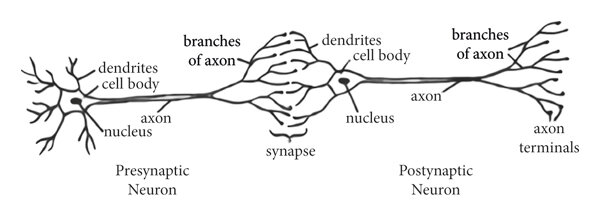
\includegraphics[width=0.8\textwidth]{BiologicalNeuron.png} % Ajuste o caminho e a largura conforme necessário
    \caption{Representação de uma rede neural biológica. Fonte: \cite{cutter2000brain}.}
    \label{fig:BiologicalNeuron}
\end{figure}

A comunicação entre os neurônios se dá por meio de sinais elétricos e químicos. Quando um neurônio recebe um estímulo suficiente, ele gera um impulso elétrico chamado potencial de ação, que se propaga ao longo do axônio até as terminações axonais. Nessas terminações, o potencial de ação provoca a liberação de neurotransmissores, substâncias químicas que atravessam a sinapse, a junção entre dois neurônios, e se ligam a receptores nos dendritos do próximo neurônio, continuando o processo de transmissão do sinal \cite{aggarwal2018neural}.

As redes neurais artificiais são formadas por neurônios artificiais inspirados nos neurônios biológicos. Esses neurônios artificiais recebem entradas (que podem ser dados ou sinais de outros neurônios), processam essas entradas através de uma função de ativação e geram uma saída. Cada entrada é multiplicada por um peso, que determina sua importância. As entradas ponderadas são somadas, resultando em uma soma ponderada. Esta soma é então passada por uma função de ativação que decide se o neurônio deve "disparar” e passar sua saída adiante na rede \cite{goodfellow2016deep}.

\begin{figure}[ht]
    \centering
    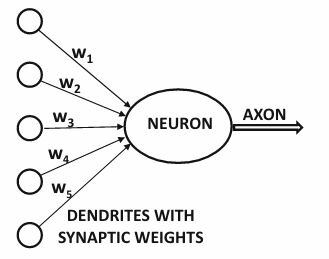
\includegraphics[width=0.8\textwidth]{ArtificialNeuron.png} % Ajuste o caminho e a largura conforme necessário
    \caption{Representação de um neurônio artificial. Fonte: \cite{aggarwal2018neural}.}
    \label{fig:ArtificialNeuron}
\end{figure}

Embora os neurônios artificiais sejam inspirados nos biológicos, eles são simplificações extremas. Os neurônios biológicos operam através de interações eletroquímicas complexas e possuem milhares de conexões com outros neurônios, enquanto os neurônios artificiais são modelados usando operações matemáticas básicas e têm um número limitado de conexões, dependendo da arquitetura da rede neural \cite{aggarwal2018neural}.

O funcionamento dos neurônios biológicos é contínuo e não linear, enquanto os neurônios artificiais geralmente funcionam de maneira discreta com uma função de ativação definida, que é muito mais simples que o comportamento real de um neurônio biológico. Essa simplificação permite que os neurônios artificiais sejam computacionalmente eficientes, embora não capturem toda a complexidade dos neurônios biológicos \cite{goodfellow2016deep}.

As redes neurais artificiais (RNAs) são sistemas computacionais inspirados na estrutura e no funcionamento do cérebro humano, projetadas para reconhecer padrões, aprender com dados e tomar decisões. Essas redes são compostas por unidades chamadas "neurônios artificiais", organizadas em camadas. As principais camadas são a camada de entrada, a camada oculta (ou camadas ocultas) e a camada de saída.

Cada neurônio recebe um ou mais sinais de entrada, que são multiplicados por pesos sinápticos. Esses sinais ponderados são somados junto a um termo de polarização, formando o valor de entrada total do neurônio, que pode ser representado pela equação \eqref{eq:linearActivation}:

\begin{equation}
    z = \sum_{i=1}^{n} w_i \cdot x_i + b
    \label{eq:linearActivation}
\end{equation}

Onde $z$ é a soma ponderada, $w_i$ são os pesos, $x_i$ são as entradas, e $b$ é o viés (ou \textit{bias}), que é um valor constante que é adicionado à combinação das entradas ponderadas para permitir o ajuste da saída do neurônio de forma mais flexível, deslocando a função de ativação \cite{goodfellow2016deep}.

O resultado $z$ é então passado por uma função de ativação $f(z)$, que determina a saída do neurônio. A função de ativação pode ser linear ou não linear, sendo as funções mais comuns a função sigmoide, ReLU (Rectified Linear Unit) e tangente hiperbólica \cite{haykin2008neural}.

A função de ativação ReLU, por exemplo, pode ser expressa de acordo com a equação \eqref{eq:ReLU}:

\begin{equation}
    f(z) = \max(0, z)
    \label{eq:ReLU}
\end{equation}

O processo de aprendizado das RNAs envolve a minimização de uma função de custo, que mede o quão longe as previsões da rede estão dos valores reais. Um método amplamente utilizado para esse ajuste é o algoritmo de retropropagação, que ajusta os pesos de cada neurônio com base no erro da saída \cite{rumelhart1986learning}. Esse ajuste é feito utilizando o gradiente descendente, onde os pesos são atualizados de acordo com a equação \eqref{eq:gradientDescent}:

\begin{equation}
    w_{i+1} = w_i - \eta \cdot \frac{\partial J}{\partial w_i}
    \label{eq:gradientDescent}
\end{equation}

Onde $\eta$ é a taxa de aprendizado e $\frac{\partial J}{\partial w_i}$ é o gradiente da função de custo em relação ao peso $w_i$ \cite{goodfellow2016deep}.

Assim, o treinamento de uma rede neural é um processo iterativo, onde os pesos são continuamente ajustados até que a função de custo atinja um mínimo, indicando que a rede foi treinada com sucesso \cite{lecun2015deep}.

Após entender a estrutura básica de uma rede neural artificial (RNA) e as funções de ativação, é importante explorar o processo de propagação e aprendizado, que inclui o \textit{forward pass}, o \textit{backpropagation}, o treinamento e a validação.

O \textit{forward pass} é a etapa em que os dados de entrada são passados pela rede, camada por camada, até que se obtenha uma previsão na camada de saída. Nessa fase, as entradas são multiplicadas pelos pesos sinápticos, somadas ao termo de polarização, e então transformadas por uma função de ativação em cada neurônio, resultando na previsão da rede. A fórmula geral para a saída de um neurônio é dada de acordo com a equação \eqref{eq:neuronOutput}:

\begin{equation}
    a = f\left(\sum_{i=1}^{n} w_i \cdot x_i + b\right)
    \label{eq:neuronOutput}
\end{equation}

Onde $a$ representa a saída do neurônio após a função de ativação, e $f$ é a função de ativação.

O processo de \textit{backpropagation} é responsável por ajustar os pesos da rede com base no erro entre a previsão da rede e o valor real. O erro é calculado usando uma função de custo, e o gradiente do erro em relação a cada peso é calculado usando a regra da cadeia. Os pesos são então ajustados na direção que minimiza o erro. O erro $E$ pode ser expresso pela função de custo, e o gradiente do erro em relação ao peso $w_i$ é dado de acordo com a equação \eqref{eq:chainRule}:

\begin{equation}
    \frac{\partial E}{\partial w_i} = \frac{\partial E}{\partial a} \cdot \frac{\partial a}{\partial z} \cdot \frac{\partial z}{\partial w_i}
    \label{eq:chainRule}
\end{equation}

Onde $a$ é a saída da rede e $z$ é a soma ponderada das entradas. A atualização do peso é feita de acordo com a equação \eqref{eq:gradientDescent}, onde $\eta$ é a taxa de aprendizado \cite{goodfellow2016deep}.

O treinamento de uma RNA envolve aplicar repetidamente o \textit{forward pass} e o \textit{backpropagation} em um conjunto de dados de treinamento, ajustando os pesos com base nos erros calculados. Este processo ocorre ao longo de várias iterações chamadas de épocas. Durante cada época, a rede processa todo o conjunto de dados de treinamento, ajustando os pesos a cada iteração. O objetivo do treinamento é encontrar o conjunto de pesos que minimize a função de custo, permitindo que a rede generalize bem para dados não vistos anteriormente \cite{lecun2015deep}.

A taxa de aprendizado $\eta$ é um parâmetro importante durante o treinamento, pois determina o tamanho dos ajustes nos pesos em cada iteração. Uma taxa de aprendizado muito alta pode fazer com que a rede oscile em torno do mínimo da função de custo, enquanto uma taxa muito baixa pode resultar em um treinamento muito lento \cite{haykin2008neural}.

A validação é um passo essencial no treinamento de redes neurais para garantir que o modelo treinado generalize bem para novos dados. Para isso, o conjunto de dados é geralmente dividido em três subconjuntos: treinamento, validação e teste. O conjunto de validação é usado para avaliar o desempenho da rede após cada época de treinamento e ajustar hiperparâmetros, como a taxa de aprendizado e a arquitetura da rede \cite{goodfellow2016deep}.

Durante a validação, a função de custo é calculada no conjunto de validação, mas os pesos não são ajustados. Isso permite verificar se a rede está começando a superajustar (\textit{overfitting}) os dados de treinamento, ou seja, aprender os ruídos ou detalhes específicos desse conjunto, em vez de captar padrões generalizáveis. Um sinal de \textit{overfitting} é quando o erro no conjunto de validação começa a aumentar enquanto o erro no conjunto de treinamento continua a diminuir \cite{nielsen2015neural}.

Ao final do treinamento, o desempenho do modelo é finalmente avaliado utilizando o conjunto de teste, que contém dados nunca vistos pela rede, fornecendo uma estimativa da capacidade de generalização do modelo \cite{goodfellow2016deep}.

\section{Aprendizado Por Reforço Profundo}

O aprendizado por reforço profundo (\textit{Deep Reinforcement Learning}, ou DRL) é uma abordagem que combina o aprendizado por reforço (\textit{Reinforcement Learning}, ou RL) com aprendizado profundo (\textit{Deep Learning}). O DRL é eficaz para treinar agentes a tomar decisões complexas e otimizar comportamentos em ambientes dinâmicos, sem a necessidade de supervisão explícita.

\subsection{Apredizado Por Reforço}

3.3.1. Aprendizado por Reforço

O aprendizado por reforço é uma abordagem de aprendizado de máquina em que um agente aprende a tomar decisões otimizadas através de interações com um ambiente. O objetivo é maximizar uma função de recompensa ao longo do tempo, ajustando suas ações com base nos feedbacks  recebidos do ambiente. O processo é definido por quatro componentes principais:

\begin{itemize}
    \item[i)] \textbf{Agente:} O sistema que toma decisões.
    \item[ii)] \textbf{Ambiente:} O contexto com o qual o agente interage.
    \item[iii)] \textbf{Ação:} As escolhas que o agente pode fazer.
    \item[iv)] \textbf{Recompensa:} O feedback do ambiente que indica a qualidade das ações do agente.
\end{itemize}

O agente segue uma política, que é uma estratégia para escolher ações com base no estado atual do ambiente. A política pode ser determinística ou estocástica. A função de valor mede a qualidade de um estado ou de uma ação, e o objetivo do aprendizado é descobrir uma política que maximize a recompensa acumulada ao longo do tempo \cite{sutton2018reinforcement}.

\subsection{Aprendizado Profundo}

O aprendizado profundo envolve o uso de redes neurais profundas para extrair características complexas e hierárquicas dos dados. As redes neurais profundas, compostas por múltiplas camadas de neurônios, são capazes de capturar representações sofisticadas dos dados e realizar tarefas como reconhecimento de imagem, processamento de linguagem natural e, mais recentemente, aprendizado por reforço.

No contexto do DRL, redes neurais profundas são usadas para aproximar funções de valor e políticas. Isso é especialmente útil em ambientes com grandes espaços de estado e ação, onde métodos tradicionais de aprendizado por reforço se tornam impraticáveis \cite{goodfellow2016deep}.

\subsection{Integração do Aprendizado por Reforço com Aprendizado Profundo}

No DRL, redes neurais profundas são empregadas para aproximar funções de valor (V(s)) e funções de ação-valor (Q(s, a)). A função de valor V(s) estima a recompensa esperada a partir de um estado s, enquanto a função de ação-valor Q(s, a) estima a recompensa esperada para uma ação a em um estado s. As redes neurais profundas permitem que essas funções sejam aproximadas de forma eficaz, mesmo em espaços de estado e ação muito grandes (Mnih et al., 2015).

Alguns dos algoritmos mais notáveis de DRL incluem:

\begin{itemize}
    \item \textbf{Deep Q-Networks (DQN):} Introduzido por Mnih et al. (2015), o DQN usa uma rede neural profunda para aproximar a função Q e é capaz de aprender políticas eficientes para uma variedade de jogos e tarefas. O algoritmo incorpora técnicas como a experiência de replay e a atualização de alvo fixo para melhorar a estabilidade do treinamento.
    
    \item \textbf{Proximal Policy Optimization (PPO):} Proposto por Schulman et al. (2017), o PPO é um algoritmo de política que busca otimizar a política de maneira estável e eficiente. O PPO é conhecido por sua simplicidade e desempenho robusto em ambientes contínuos e discretos.
    
    \item \textbf{Trust Region Policy Optimization (TRPO):} Desenvolvido por Schulman et al. (2015), o TRPO melhora a estabilidade do treinamento de políticas ao garantir que as atualizações da política não desviem muito da política anterior.
\end{itemize}

O DRL tem sido aplicado em uma ampla gama de áreas, incluindo:

\begin{itemize}
    \item \textbf{Jogos:} O DRL tem alcançado sucesso em jogos complexos como o Atari, Go e StarCraft II, demonstrando a capacidade dos agentes para aprender e otimizar estratégias avançadas \cite{silver2016mastering}.
    
    \item \textbf{Robótica:} Em robótica, o DRL é utilizado para ensinar robôs a realizar tarefas complexas, como manipulação de objetos e navegação em ambientes desconhecidos \cite{lillicrap2016continuous}.
    
    \item \textbf{Controle de Sistemas:} O DRL também é utilizado para otimizar o controle de sistemas em tempo real, como a gestão de redes elétricas e sistemas de tráfego \cite{mnih2015human}.
\end{itemize}
\chapter[Metodologia ou Materiais e Métodos]{Metodologia ou Materiais e Métodos}\label{capitulo4}
\addcontentsline{toc}{chapter}{Metodologia ou Materiais e Métodos}
\chapter[Desenvolvimento]{Desenvolvimento}\label{capitulo5}
\addcontentsline{toc}{chapter}{Desenvolvimento}
\chapter[Cronograma]{Cronograma}\label{capitulo6}
\addcontentsline{toc}{chapter}{Cronograma}

\begin{table}[ht]
    \centering
    \caption{Cronograma}
    \begin{adjustbox}{max width=\textwidth}
    \begin{tabular}{|p{5cm}|c|c|c|c|c|c|c|c|c|c|}
        \hline
        Atividade & MAR & ABR & MAI & JUN & JUL & AGO & SET & OUT & NOV & DEZ \\
        \hline
        \parbox[t]{5cm}{\textit{Brainstorming} e \\ desenvolvimento inicial \\ da ideia} & X & X &  &  &  &  &  &  &  &  \\
        \hline
        \parbox[t]{5cm}{Pesquisa e revisão \\ de literatura} &  & X & X & X & X & X &  &  &  &  \\
        \hline
        \parbox[t]{5cm}{Criação da parte escrita \\ do TCC 1} &  &  &  &  & X & X &  &  &  &  \\
        \hline
        \parbox[t]{5cm}{Desenvolvimento da \\ rede neural e do jogo} &  &  &  &  &  & X & X & X & X &  \\
        \hline
        \parbox[t]{5cm}{Testes com outras \\ pessoas} &  &  &  &  &  &  &  & X & X &  \\
        \hline
        \parbox[t]{5cm}{Criação da parte escrita \\ do TCC 2} &  &  &  &  &  &  &  &  & X & X \\
        \hline
    \end{tabular}
    \end{adjustbox}
    \label{tab:tabela11x6}
\end{table}
\chapter[Trabalhos Futuros]{Trabalhos Futuros}\label{capitulo7}
\addcontentsline{toc}{chapter}{Trabalhos Futuros}

\section{Trabalhos Futuros}

% ----------------------------------------------------------
% ELEMENTOS PÓS-TEXTUAIS
% ----------------------------------------------------------
\postextual
% ----------------------------------------------------------

% ----------------------------------------------------------
% Referências bibliográficas
% ----------------------------------------------------------
\bibliography{bibliografia}

% ----------------------------------------------------------
% Glossário
% ----------------------------------------------------------
% Consulte o manual da classe abntex2 para orientações sobre o glossário.
%\glossary

% Apêndices
\begin{apendicesenv}

% Imprime uma página indicando o início dos apêndices
\partapendices

\chapter{1}
Texto

\chapter{2}
Texto

\end{apendicesenv}
% ---
% Anexos
\begin{anexosenv}

% Imprime uma página indicando o início dos anexos
\partanexos

\chapter{1}
Texto

\chapter{2}
Texto

\chapter{3}
Texto

\end{anexosenv}

%---------------------------------------------------------------------
% INDICE REMISSIVO
%---------------------------------------------------------------------
\phantompart
\printindex
%---------------------------------------------------------------------

\end{document}
